%%%%%%%%%%%%%%%%%%%%%%%%%%%%%%%%
\section{Overview}
\label{sec:detectors-fd-ref-ov}


This chapter describes the reference design of the DUNE far detector.  The detector will consist of four nominal 10-kt fiducial mass, single-phase liquid argon time projection chambers (TPCs) augmented with a photon detection system.  A ``Single-phase'' detector is one in which the charge generation, drift and collection all occur in liquid argon (LAr). The scope of the far detector includes the design, procurement, fabrication, testing, delivery, installation and commissioning of the detector components: 

\begin{itemize}
\item Time Projection Chamber (TPC)
\item Data Acquisition System (DAQ)  
\item Cold Electronics (CE)
\item Photon Detector System (PD)
\end{itemize}
The TPCs will be housed in cryostats provided by LBNF, described in \vollbnf. The reference design is based largely on the LBNE far detector design as of January 2015, documented in \anxlbnefd. This annex provides the detailed descriptions of the systems and components that the DUNE reference design incorporates; the differences between the DUNE and LBNE designs are clearly indicated in this chapter. Important differences include detector size, APA and CPA placement, and small changes to the APA dimensions.


The detector modules are planned to be constructed in a staged fashion with the first module coming online as soon as possible and the rest at a regular pace. A model of the underground experimental area with the four 10-kt detector modules is shown in Figure~\ref{fig:FarDet-overview-SP}. Planning for the conventional facilities calls for construction of the second cryostat to be completed prior to filling the first so that it may serve initially as a liquid storage facility. 
The detector technology is expected to improve in the coming years with MicroBooNE, the SBN experiment and the CERN neutrino-platform development program. DUNE's staged program allows selection of the optimal design for each module as the technology evolves.  %detector module at each step. 

\begin{cdrfigure}[FD overview reference design]{FarDet-overview-SP}{Left: 3D model of the reference design for the DUNE far detector to be located at the 4850L. Right: Schematic view of the active detector elements showing the plane ordering of the TPC inside the detector.}
\centering
\begin{minipage}[b]{1.0\textwidth}
\begin{center}
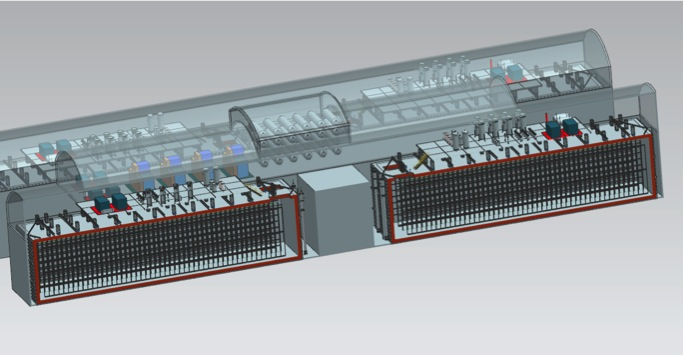
\includegraphics[width=.58\textwidth]{FarDet-3D-SP.jpg}
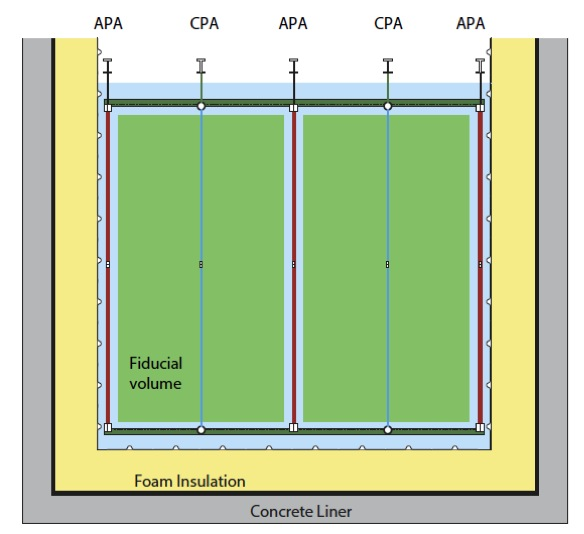
\includegraphics[width=0.38\textwidth]{FarDet-endview-SP.jpg}
\end{center}
\end{minipage}
\end{cdrfigure}

The reference design, presented in this chapter and documented in the project cost and schedule, is  
patterned after the successful ICARUS experiment, but adapted to the local site requirements at SURF and the need to scale up the detector size. The configuration of the TPC detector is shown on the right in Figure~\ref{fig:FarDet-overview-SP}.  The TPC, described in Section~\ref{sec:detectors-fd-ref-tpc}, is constructed by placing alternating high-voltage cathode planes and anode readout planes in a bath of ultra-pure liquid argon. Particles interacting in the argon generate charge and vacuum ultra-violet (VUV) photons. 


The single-phase design offers the advantage that the charge is collected directly, enabling precision charge calibration. However, signal levels are low, requiring the use of cold electronics (Section~\ref{sec:detectors-fd-ref-ce}), and the readout is based on stereo induction planes, requiring a de-convolution of the induced signal. A photon detection system (Section~\ref{sec:detectors-fd-ref-pd}) provides the t$_0$ or event time for physics processes uncorrelated with the FNAL neutrino beam.



The expected performance of the DUNE far detector is based on the measured performance of the ICARUS detector, scanned Monte Carlo events and newer studies with automated reconstruction. The requirements and projected performance are summarized in Table~\ref{tab:TPC-metric}. It is expected that as the software tools improve and as measurements from MicroBooNE and other dedicated test-beam programs become available the uncertainties on the projected performance will become smaller.

\begin{cdrtable}[DUNE Far Detector Performance Expectations]{llll}{TPC-metric}{Summary of the most important performance parameters of the DUNE reference far detector. Included are the parameters, previous detector performance, and projected performance with references to relevant studies.} 
%The third argument (reads {cc}) can use c, l, r or p{some length}  e.g. {clll} or {llp{3cm}}, for instance.
Parameter & Requirement & Achieved Elsewhere & Expected Performance \\ \toprowrule
Signal/Noise Ratio\footnote{For a MIP at the CPA, minimum in all three views, for any track angle} & 9:1 & 15:1~\cite{Antonello:2015zea,Antonello:2014eha} & 9:1 \\ \colhline
Electron Lifetime & 1.5~ms & $>15$~ms~\cite{Antonello:2014eha} & $>1.5$~ms \\ \colhline
Uncertainty on Charge & & & \\
Loss due to Lifetime  &   $<1\%$  & $<1\%$~\cite{Antonello:2014eha} & $<1\%$ \\ \colhline
Two-Hit Resolution & 2~mm & & 2~mm \\ \colhline
Track-Finding Efficiency\footnote{For tracks with $L>5$~cm} & $>98\%$ & & $>98\%$ \\ \colhline
Vertex Position Resolution & (0.5,0.8,0.2)~cm & & (0.5,0.8,0.2)~cm \\ \colhline
$e-\gamma$ separation $\epsilon_e$ & 0.9 & & 0.9 \\ \colhline
$e-\gamma$ separation $\gamma$ rejection & 0.99 & & 0.99 \\ \colhline
Multiple Scattering Resolution & & & \\
on muon momentum\footnote{For a sample of stopping muons} & 18\% & 18\%~\cite{gibinmuon,Ankowski:2006ts} & 18\% \\ \colhline
Electron Energy Scale & & & From LArIAT \\
Uncertainty & 1\% & 2.2\%\cite{ICARUS-pizero} &  and CERN Prototype \\ \colhline
Electron Energy Resolution & $0.15/\sqrt{E{\rm (MeV)}}$ &$0.33/\sqrt{E{\rm (MeV)}}$  \cite{ICARUS-pizero} & From LArIAT \\
 & $\oplus 1\%$ & $\oplus 1\%$ & and CERN Prototype \\ \colhline
Energy Resolution for & & & \\
Stopping Hadrons & 1-3\% & & 1-3\% \\ \colhline
Stub-Finding Efficiency\footnote{For electron stubs with $E>5$~MeV} & 90\% & & \\ \colhline
Stub Arrival Time Resolution & 0.1~ms & & \\
\end{cdrtable}
